\documentclass{aa}
% \documentclass[referee]{aa}
% \documentclass[bibyear]{aa} 
\usepackage[varg]{txfonts}
\bibpunct{(}{)}{;}{a}{}{,}
\usepackage{graphicx}
\usepackage{algorithm}
\usepackage[noend]{algpseudocode}
\usepackage{cellspace}
\usepackage{url}
\usepackage[toc, page]{appendix}
\usepackage[utf8]{inputenc} %unicode support

\begin{document}
\title{On the identification of Earth-impacting asteroids using an artificial neural network}
\author{John D. Hefele\inst{1}
\and Francesco Bortolussi\inst{2}
\and Simon Portegies Zwart\inst{3}}
\institute{Sterrewacht, Leiden University, Leiden, NL
\and LIACS, Leiden University, Leiden, NL
\and Sterrewacht, Leiden University, Leiden, NL}
\date{Received DD MM YYYY / Accepted DD MM YYYY}
\abstract{We identify potentially Earth impacting asteroids by means of an artificial neural network. We name the resulting
instrument the Hazardous Object Identifier (or HOI for short). The
network is trained on an artificial set of known impactors which was
generated by launching objects from Earth's surface and integrating
them backwards in time. HOI was able to identify
95.25\% of \textbf{the simulated known-impactors present in the test set as potential-impactors}. \textbf{HOI was additionally able to identify 90.99\% of the potentially hazardous objects, as identified by NASA, without being trained on them. HOI also} identified 99.9\% of objects that approached within 0.05\,au of Earth in the coming thousand years.}
\keywords{Comets: general - Minor planets, asteroids: general - Methods: data analysis - Methods: statistical}
\titlerunning{On the identification of Earth-impacting asteroids using an artificial neural network}
\authorrunning{J. D. Hefele et al.}
\maketitle


\section{Introduction}
\label{SEC:Introduction}
In 1990, the US Congress requested for NASA to establish two workshops
to focus on the identification of potentially hazardous small bodies
and on methods to alter their orbits to prevent an impact
\citep{milani2002}. The workshops led to the establishment of the
\textit{Sentry: Earth Impact Monitoring} system \citep{Sentry}.  If a
hazardous asteroid would be identified sufficiently early before
impact, it would be possible to mitigate the impact by means of an
appropriate space mission to alter the asteroid's orbit through a
gravitational tugboat \citep{10.2307/26060526}, or by obliterating it
with a nuclear warhead \citep{BARBEE201837}.  Both mitigation
strategies require many years of preparation, which makes the early
detection of hazardous objects vital to allow ample time for
mission preparation.

The Sentry system adopts a Monte Carlo approach in which millions of
virtual objects are launched with orbital parameters statistically
sampled from within the error ellipse of the observed asteroids. The
impact probability is subsequently determined on the fraction of
virtual asteroids that reach Earth within some pre-determined striking
distance \citep{milani2002}. In this approach, the orbits of many
asteroids are integrated numerically and the final parameter space is
considered to represent the probability-density distribution of the
respective objects. The calculation of this probability density
distribution relies on the algorithm and implementation used to
integrate the orbits of the asteroids.  The time scale over which such
integrations remains reliable depends on the degree by which the
asteroid's orbit is chaotic, i.e. on the value of the largest positive
Lyapunov exponent.  Additionally, the reliability of such integrations
depends on the ability of the integrator to obtain a solution, such that the integration complies to the concept of {\em
  nagh Hoch}\footnote{\textbf{\textit{Nagh Hoch} is the concept that an ensemble of random initial realizations in a wide range of parameters gives statistically the same result as the converged solutions of the same ensemble realizations.}}
\citep{PORTEGIESZWART2018160}.  
\par
\textbf{Both} of these concepts are not
guaranteed with the adopted numerical schemes, and the results reach
questionable proportions as soon as the asteroid experiences a close
encounter with any object other than the Earth. In the latter case,
the phase space of possible solutions grows exponentially due to the
chaotic nature of the equations of motion.  Establishing the chaotic
nature of an asteroid is limited by the accuracy of its orbital
determination. This is generally realized by observing any particular
asteroid a number of times. These observations result in a data arc,
the fraction of the orbit over which the object has been observed.
The adopted Monte-Carlo method used in the Sentry system is expected
to be reliable for at most a few dozens of years
\citep{HorizonsManual} for asteroids for which the observed data arc
is smaller than a month, which is 12.9\% of all small-bodies \citep{dastcom5}.

Considering the high degree of chaotic motion (small Lyapunov time
scale) in asteroids and its consequential exponential divergence of
its orbit, one can wonder if it is worth the effort to perform
extensive computer simulations in order to track the orbital
trajectories of a large number of particles so long as the veracity of
the orbital integration can not be guaranteed. For the most chaotic
asteroids, the impact probability sensitively depends on the
statistics of the adopted method and a more coarse grained approach to
identify potentially hazardous objects may suffice. This approach
would free-up computer time to provide a more reliable impact probability for the most promising candidate impostors. 

We explore the population of asteroids, and in
particular the potentially dangerous ones, by means of automatic
machine recognition through a combination of numerical integrations and
a trained neural network \textbf{similar to the architectures described in \citep{ref1} and \citep{ref2}, which were used for classifying hazardous taxonomy and solar sail transfer time estimation}. It is a statistical approach in which we
determine the prospect for impact of the known population of asteroids
gathered from the \textit{dastcom5} off-line database \citep{dastcom5}.  Our
analysis is mediated by \textbf{an artificial neural-network} dubbed HOI\footnote{This also means ``Hello'' in the Dutch language.} for ``Hazardous Object Identifier'', which was trained
on a population of known-impactors (KI) and a random sample from the
observed database using \textbf{the \textit{TensorFlow} framework} \citep{TensorFlow}. The KIs are machine generated from an integrated
population of asteroids that start their orbit on a random position of
Earth's surface and are launched radially away with the planet's escape
speed. These objects are subsequently integrated backwards in time
together with the planets in the Solar system for up to 20,000
years. To train HOI, these computer generated KIs are then mixed with a subset of observed asteroids, which we assume to be known non-impacting objects. The trained network is then used on another random selection of observed asteroids
in order to identify potential impactors (PIs). \textbf{All the objects that were not identified by the model as PIs, and that were not initially labeled as KIs, are referred to as unidentified objects (UOs).}

We begin by describing HOI's architecture in section\,\ref{SEC:1D_CNN}, which is followed by a discussion of the generation of the small-body datasets in section\,\ref{SEC:Data}. The results are examined in section\,\ref{SEC:Results} and conclusions are drawn in section\,\ref{SEC:Conclusions}. All the code
used to train the neural network, generate data, and evaluate the
results are publicly available on \textbf{GitHub}\footnote{ \url{https://github.com/mrteetoe/HOI}}.
%\citep{koon,oreg,khar,zvai,xjon,schn,pond,smith,marg,hunn,advi,koha,mouse}

\section{HOI's architecture}
\label{SEC:1D_CNN}

In general, \textbf{neural networks} are particularly well suited for
recognizing complex patterns hidden in \textbf{multi-dimensional datasets}. In our particular case, we strive to identify observed objects that have topologically similar trajectories to the trajectories of the population of known hitters. \textbf{Because we are no longer reliant on calculations that attempt to estimate the asteroids position at a particular point in time, the network is more resilient to perturbations of the initial conditions i.e. chaotic motion.}

The problem at hand is a discrete binary classification task, where the two mutually exclusive classes are either \textbf{ ``potential impactors'' (PIs) or ``unidentified objects'' (UOs). For the purpose of our experiments, the UOs are what we would consider ``benign objects'', i.e. objects that are not regarded as PIs}. To quantify the network's accuracy, the standard ``cross entropy'' cost function is used. This can be defined as follows:
\begin{equation}
	\label{cost_function}
	H(y,\hat{y})=-\sum_i^{N} y_i \text{ln}(\hat{y}_i)+(1-y_i)\text{ln}(1-\hat{y}_i)
\end{equation}
Here $y$ is the actual value, or label, $\hat{y}$ is the predicted value, and $N$ is the total amount of predictions. This cost function has the convenient property that its derivative with respect to some input weight, $w$, scales linearly with the difference between the label and predicted value \citep{Nielson}:
\begin{equation}
	\frac{\partial C}{\partial w}=\frac{1}{N}\sum^{N}_i x(\hat{y}_i-y_i)
\end{equation}
Here $x$ is the input value by which $w$ is multiplied. To minimize (\ref{cost_function}), the ``Adam Optimizer'' is used, which expands upon na\"{i}ve stochastic gradient descent by adapting its learning rate based on both the average of the first and second moments of the gradients \citep{AdamOptimizer}. Empirically, it is observed that this optimizer reduced the cost function to the lowest value with the fewest number of iterations relative to the other algorithms available in TensorFlow. 
\par 
    Each object fed into HOI is represented by a \textbf{5 element vector where each vector} are the Keplerian elements of the asteroids around the sun including the semi-major axis (\textit{a}), eccentricity (\textit{e}), inclination (\textit{i}), the mean speed (\textit{N}), and the specific angular momentum (\textit{H}).
    \textbf{These 5 orbital elements fully characterize of the shape and orientation of an asteroid trajectory around the sun.}
\par 
A diagram of HOI's architecture is shown in figure \ref{FIG:HOI_Design}.
\begin{figure}[t]
    \hspace*{-0.4cm}
	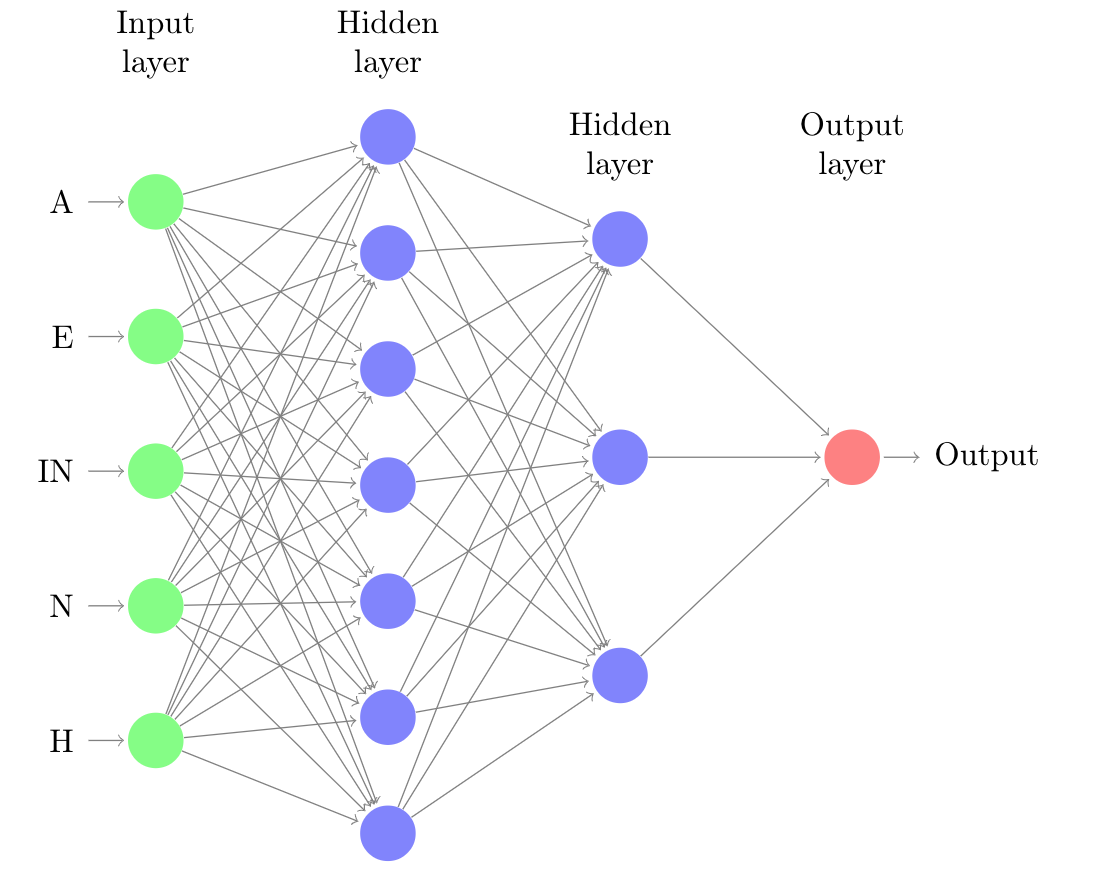
\includegraphics[width=83mm]{images/1_network_hoi.png}
	\centering
	\caption{\label{FIG:HOI_Design} \textbf{HOI network architecture. The input layer is comprised of 5 nodes, which is followed by two hidden layers of 7 and 3 nodes and an output layer of a single node}.}
\end{figure}
The input layer is a \textbf{vector of $5$ neurons to match the dimensionality of the input, which is followed by two hidden layers that are composed of 7 and 3 neurons respectively from the input layer. The output is a single neuron whose values are restrained between 0 and 1 by virtue of the sigmoid function where objects with a rating of 0.5 or above are classified as PI and those below the threshold are classified as UO.  This neural network architecture was arrived at by experimentation. We wanted to provide the network with enough degrees of freedom to properly generalize the orbital elemental profiles of KI but not to give it so many degrees of freedom that the network would overfit to the training datasets}.    
\par  
The described architecture results in \textbf{69} free parameters: \textbf{59 weights and 10 biases} \footnote{Following the architecture described, the number of free parameters can be calculated as follows: \textbf{the input is fed through layers which are comprised of 7, 3, and 1 neuron(s). This results in 5$\times$7+7$\times$3+3$\times$1 weights and 7+3 biases, as only the hidden layers have bias parameters}.}. To optimize these parameters, the network is trained on 5 randomly selected sub-sets of 100,000 observed and KI objects over \textbf{28 epochs, which took less than 5 minutes on a CPU-type laptop without a GPU. The training was halted when the relative loss decrease per epoch was less than $1\%$, to prevent overfitting At the end of the training process the network's performance is validate with a subset of 20,000 KI and 20,000 observed objects that were held out of the training process}. Furthermore, all potentially hazardous objects (PHOs)\footnote{All objects with a minimum orbit intersection distance of 0.05 AU or less and an absolute magnitude (H) of 22.0 or less are considered PHOs \citep{NasaPHA}.} are held out of the training process and used exclusively for testing purposes. \textbf{Figure \ref{FIG:loss} shows how the loss decreases while the fraction of PHO hazardous objects identified simultaneously increases.}
\par
We gave the observed objects and KIs labels of 0.1 and 0.9 respectively. Here, higher numbers correspond with a greater chance of colliding with Earth meaning that the observed objects as a whole are assumed to have a negligible impact probability. 
\textbf{The labels are chosen as such to represent the fact that we are not certain that all the observed objects will not impact Earth and that KI trajectories are not calculated with infinite precision so that it cannot be guaranteed that these objects will collide with Earth when their velocities are reversed.}  

It is a safe to assume that any individual observed object is benign considering that impacts from large objects are rare \citep{Chapman} and that the impact frequency of an asteroid collision decreases with the cube of an asteroid's diameter: Earth collisions with 5-kilometer asteroids occur approximately every 20 million years while those with a 100 meter asteroids occur every 500 years \citep{Bostrom}. Because 98.4\% of the observed objects used for our experiments are greater than 100 meters in diameter\footnote{This assumes that an absolute magnitude of 22.5 corresponds to a 100-meter diameter, which can be calculated by using equation \ref{HtoDiameter} and assuming an albedo of 0.15} we can use the following formula to estimate an upper-bound of the number of expected Earth impacts from asteroids in our sample within the next 20,000 years:
\begin{equation}
    N_{collisions}=\int^{\infty}_{100}\frac{4\times10^7}{D^3}=2000
\end{equation}
Here, $D$ are the asteroids' diameters. This simple calculation does not take into account that many of the existing asteroids have not yet been observed and stored in the \textit{dastcom5} database. Additionally, all of the PHOs, which have considerably higher chances of collision than the rest of the observed population, are not used in HOI's training and therefore are not mislabeled. Because of this, at the very most, only 0.3\% of the observed objects are mislabeled. However, this percentage is likely considerably lower and is nonetheless small enough not to have a negative impact on HOI's performance.  
\begin{figure}[t]
	\hspace*{-0.3cm}
 	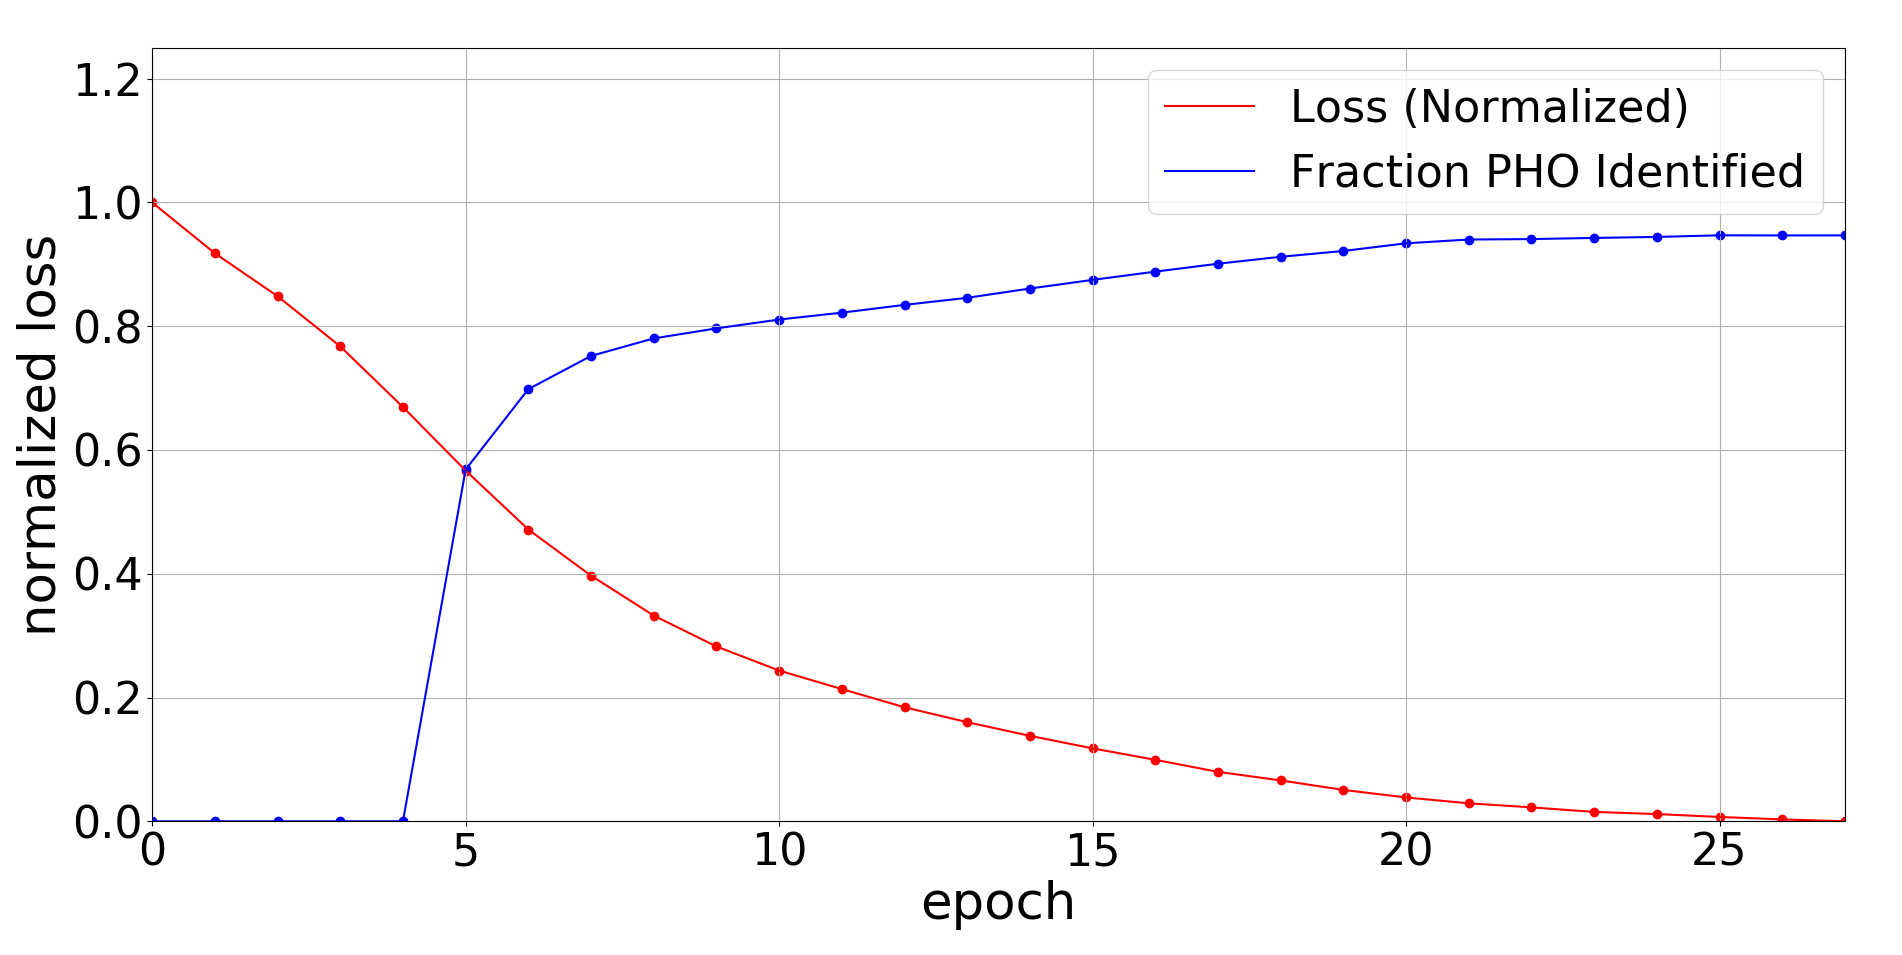
\includegraphics[width=83mm]{images/cost_epoch_pho.png}
	\centering
	\caption{\label{FIG:loss} Plot of the loss and fraction of PHOs identified versus the epoch number during the training phase.}
\end{figure}

\label{SEC:KnownImpactors}
\section{Data generation and acquisition}
\label{SEC:Data}
\subsection{Observed objects}
\label{SEC:RealAsteroids}
736,496 small bodies are extracted from NASA's \textit{dastcom5} database, which is a ``portable direct-access database containing all NASA/JPL asteroid and comet orbit solutions used by the NASA/JPL Horizons ephemeris system'' \citep{dastcom5}. Roughly 95.5\% of the extracted objects are main belt asteroids, 3.2\% are asteroids that are not in the main belt (such as Apollo or Trojan asteroids), 0.7\% are comets, 0.2\% are Kuiper Belt Objects (KBOs), and the remaining 0.4\% of the small bodies are composed of a plethora of miscellaneous objects such as planetary satellites and centaurs \citep{SolarSystemObjects}. It is worth noting that these proportions are most likely not representative of the actual small-body populations as there is an observational bias towards the closer main-belt asteroids in comparison with the far-flung KBOs \citep{KBO_Population}.

\textbf{paragraph was removed because it is irrelevant in consideration of the other revisions}
 
%Considering that some objects would approximately have a number of virtual asteroids generated comparable to the total number of observed objects to compute a single collision probability via the Monte-Carlo approach highlights the method's humongous computational demands and the need of a faster approach. 

\subsection{The known impactors}

To act as examples of hazardous objects, we generate an ensemble of 800,000 KIs by launching asteroids from future positions of Earth's surface and them integrating backwards in time to the year 2020.
However, for training/testing the network we use only 330,000 of these objects because over half of the KIs either left the solar system, were unable to escape Earth's gravitational field, or spun into the Sun. The procedure used to generate the KIs is outlined in Algorithm \ref{generate-ki}.

The future launch dates are evenly distributed between the years 2318 and 22018 for the 8,000 simulations performed ($800,000/100$). This corresponds to a spacing of approximately two and half years between future launches, a minimum integration time of 300 years, and a maximum integration time of 20,000 years. \textbf{We generate the KI in batches of 100 because it was observed that larger batches cause the simulations to run considerably slower}.
 
An object, for example, that is launched from the solar system at the year 2318, and is then integrated backwards in time 300 years, would create an example of a present day asteroid that would strike the Earth in 300 years after the velocity vectors are negated to account for time reversal. Therefore, the length of a KI's backward integration directly corresponds with its expected impact date with Earth. 

\begin{algorithm}[h]
\caption{Observed asteroids forward-integration}\label{generate-ki}
\begin{algorithmic}[1]
\State{Until all trajectories are calculated:}
        \For{batch of 100 objects}
            \State \parbox[t]{\dimexpr\textwidth-\leftmargin-\labelsep-\labelwidth}{Initialize the sun, moon and planetary positions and \\ velocities}
            \State{Integrate them forward in time}
            \State \parbox[t]{\dimexpr\textwidth-\leftmargin-\labelsep-\labelwidth}{Launch 100 objects from random positions on the \\ Earth's surface over the course of 1 Jupiter period \\ radially with velocities with a flat distribution between \\ 15 and 45km/s.}
            \State \parbox[t]{\dimexpr\textwidth-\leftmargin-\labelsep-\labelwidth}{Integrate all objects backwards in time until the year \\ 2018.}
            
\EndFor
\end{algorithmic}
\end{algorithm}

The launching velocities are selected to bracket the Earth's and Solar System's escape speeds of 11.2 km/s and 42.5km/s respectively. The majority of objects launched outside this range either get trapped in the Earth's gravitational field or leave the solar system within one orbit. We deliberately do not attempt to mimic the observed asteroid impact velocities to allow the neural network to learn from the full range of parameters rather than on a hand-selected subsample. 

\textbf{Simulating the KIs does not present clear limitations: although the trajectories of the simulated asteroids are computed with a finite bit precision, which introduces inaccuracies, the derived orbital parameters of any observed objects are never without uncertainties. Therefore, if a large collection of observed orbital parameters were available from a set of objects that collided with Earth, this dataset would provide no better examples of hazardous objects to HOI than what is currently provided by the generated KIs.}

\section{Results}
\label{SEC:Results}

\textbf{paragraph was removed because it is irrelevant in consideration of the other revisions}

Following the procedure described in \S\,\ref{SEC:1D_CNN}, and testing on all of the objects that the network was not trained on, leads to 95.25\% of KI, 90.99\% of PHOs and 1.94\% of observed objects being classified as PIs. The high percentage of correctly identified KIs proves that HOI can identify nearly every object that will strike Earth or come close to it \footnote{Because the simulations are not performed with infinite precision, it is not guaranteed that all KIs will collide with the Earth when they are integrated forward in time.}. This performance should be expected considering that HOI was specifically tuned to identify artificial KI objects. A more meaningful metric of performance is the percentage of PHOs identified. Although \textbf{9.01\% PHOs were not identified, HOI is approximately 47 (90.99/1.94) times more likely to select a PHO over some other observed object}.
% The most hazardous objects as classified by Sentry: 2009 FD, Bennu, and 1950 DA, are all identified by HOI as PIs, which have impact probabilities of 1.6e-3, 3.7e-4, and 1.2e-4 respectively \citep{Sentry}. 
 
To further evaluate the effectiveness of HOI, simulations are performed to compare the closest approaches of PIs to UOs relative to Earth. The algorithm utilized to perform these calculations is the same in every respect to the Algorithm \ref{generate-ki} with the exception that each object is integrated forward in time for 1,000 years. The trajectories of all 14,680 PIs and an equal amount of unselected observed objects are computed. The closest approaches achieved during these integrations are shown in figure \ref{FIG:Closeness_Histogram} with the exception of 108 PIs and 884 unselected observed objects, as their closest approaches exceeded the x-axis limits of 2 \,au. Virtually every object that got within 0.01\,au of Earth and 99.9\% of objects that got within 0.05\,au of Earth are identified by HOI as PIs. 
\begin{figure}[h]
	\hspace*{-0.35cm}
	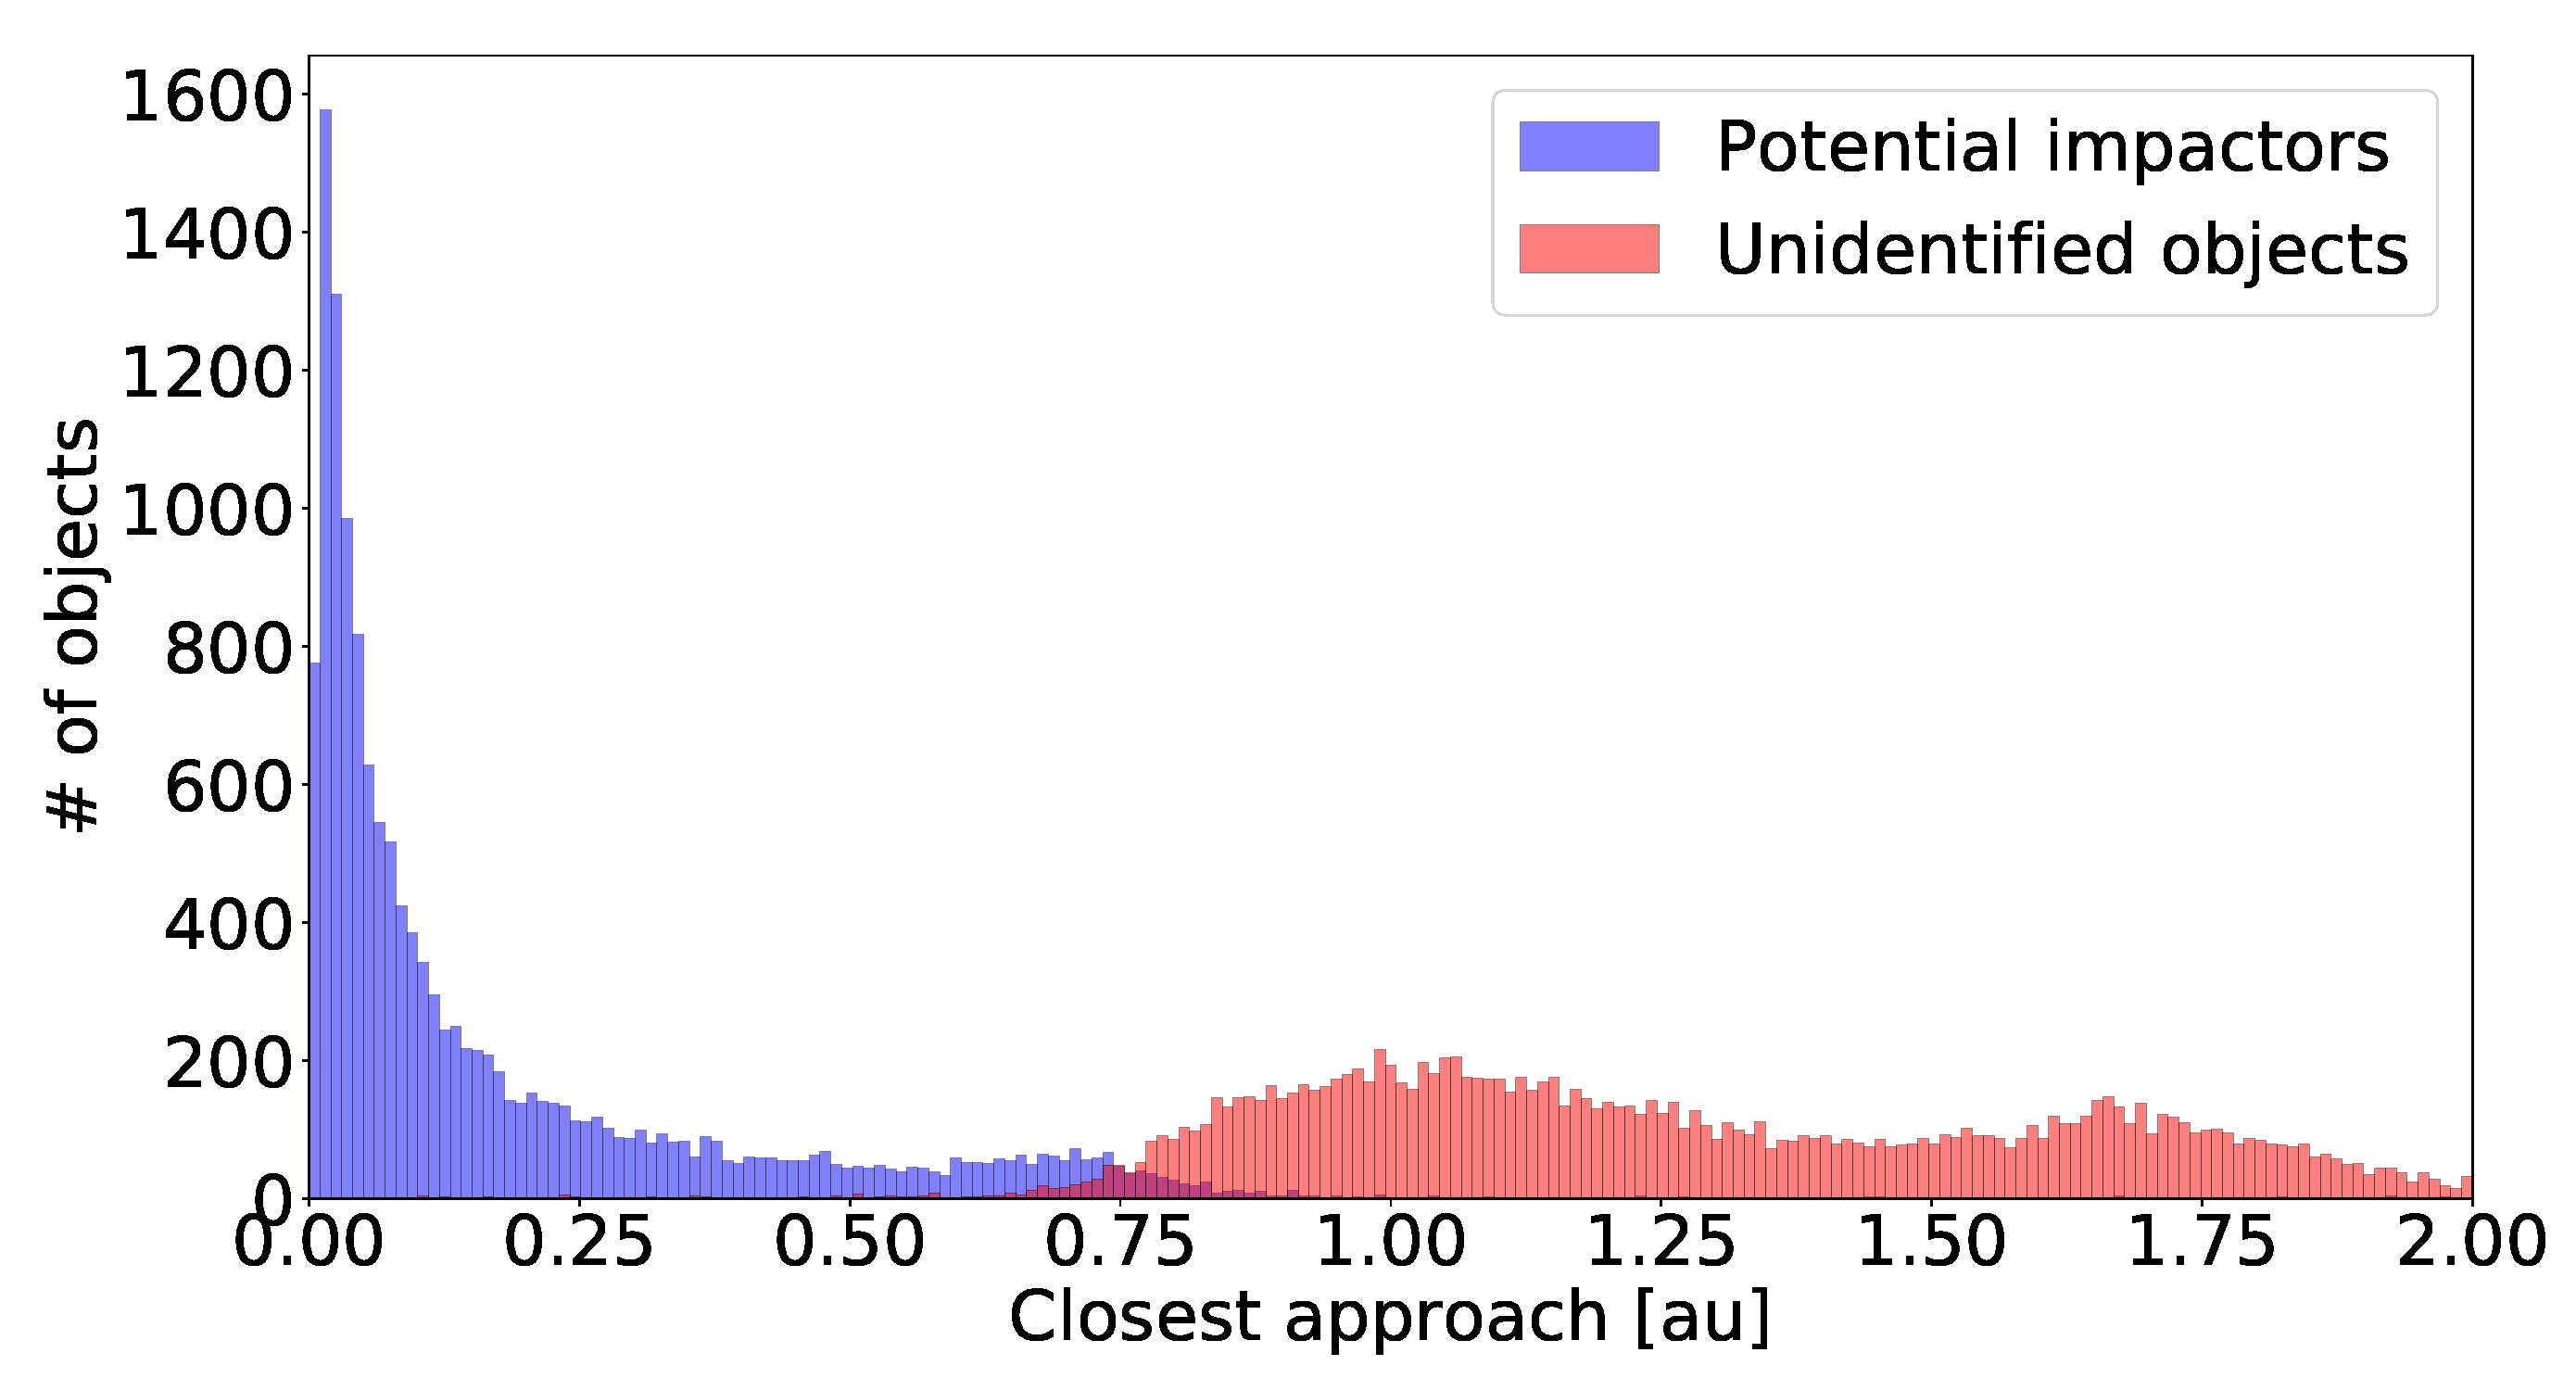
\includegraphics[width=83mm]{images/3_Closest_Approach_Together.pdf}
	\centering
	\caption{\label{FIG:Closeness_Histogram} Plot of the  the shortest distances from Earth calculated when PIs and benign observed objects were integrated 1,000 years into the future}
\end{figure}
 
To investigate why HOI only identifies approximately nine-tenths of PHOs as PIs, the thousand-year integrations described above are additionally performed on all unidentified PHOs. A histogram depicting these closest approaches are shown in figure \ref{FIG:Closeness_PHOs}. The distributions of identified PHOs and unidentified PHOs are similar. Because of this, the percentage of PHOs \textbf{classified as PIs} could be used as a measure of the network's performance, as ideally all of them should have been identified. Additionally, all objects that did not approach Earth within at least 0.5\,au could be considered misclassified PIs. This cut-off is not arbitrary, but is rather based on the minimum distance achieved by 99.7 percent, or $2\sigma$, of PHOs. In the case of HOI, 12.2\% of the PIs are outside of this threshold \textbf{ and can be safely considered misclassified. The root of this misclassification likely stems from the fact that not all of the KIs will collide with Earth when integrated forward in time and that all of the observed objects are in fact not benign, which implies that the labeling scheme used to train HOI is imperfect.}
\begin{figure}[h]
    \hspace*{-0.44cm}
	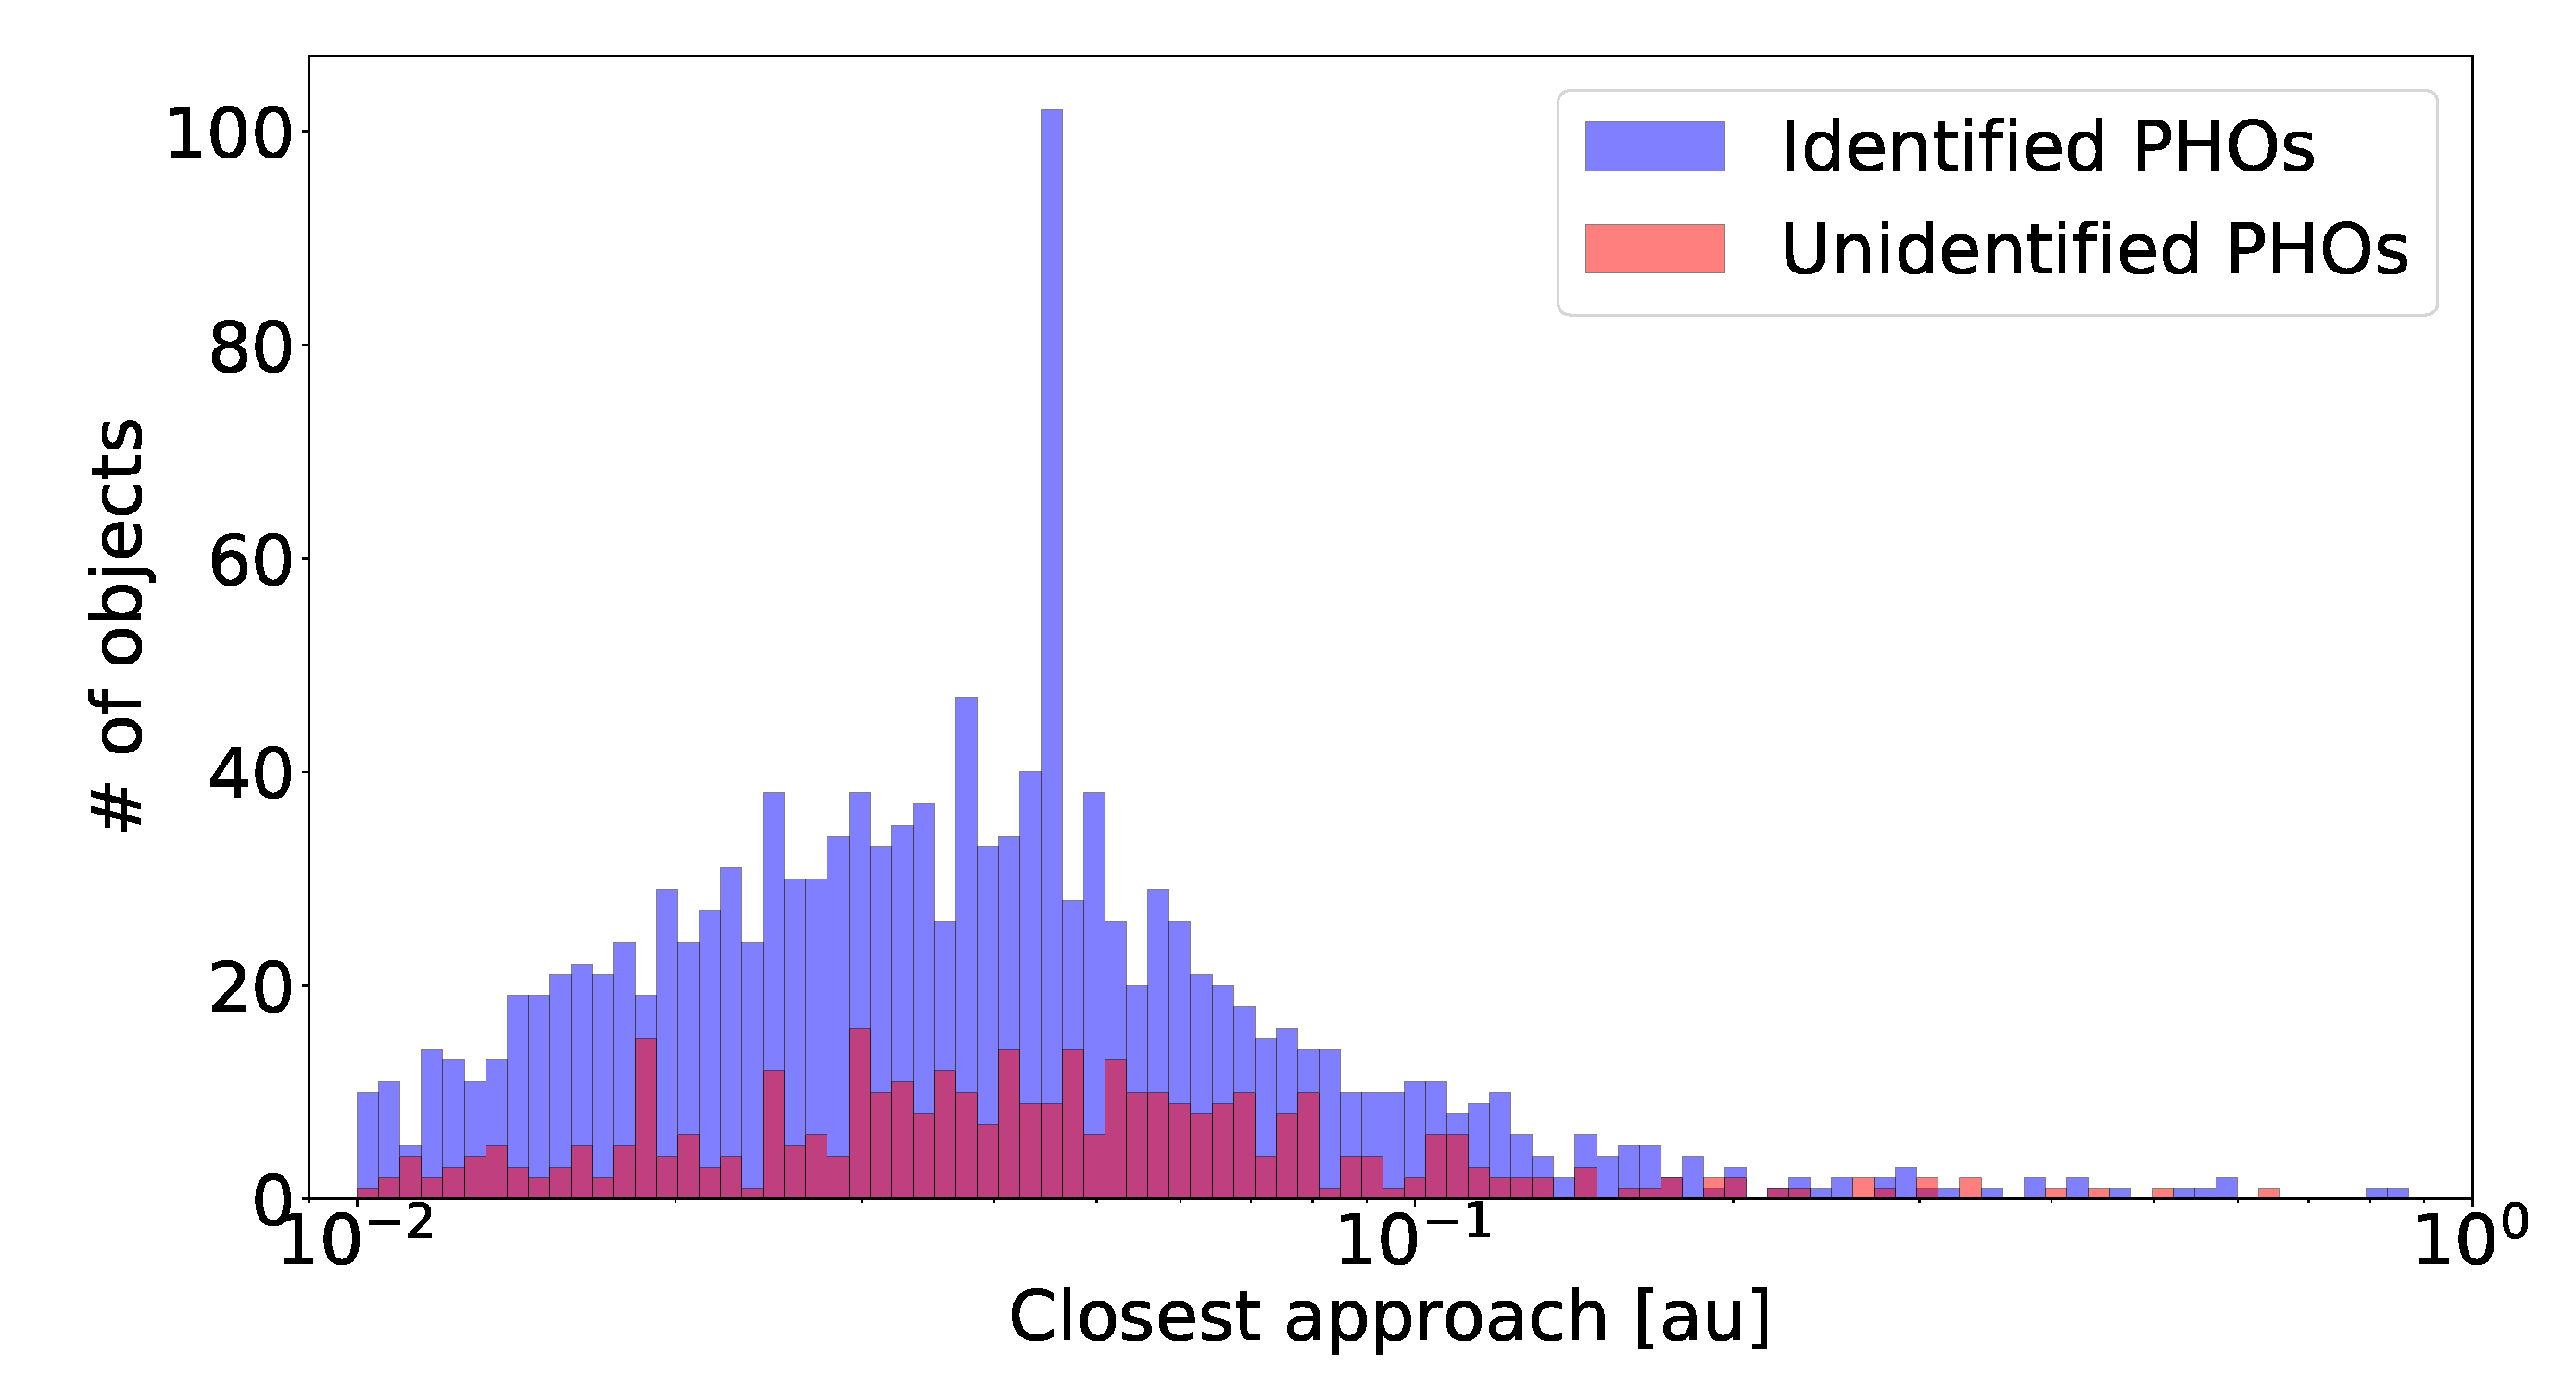
\includegraphics[width=85mm]{images/4_Closeness_Plots_PHOsLog.pdf}
	\centering
	\caption{\label{FIG:Closeness_PHOs} Illustrates the closest approaches achieved in the thousand year simulations of PHOs that were identified by HOI and those that were not.}
\end{figure}

13,258 of the bodies classified as KIs are not listed as PHOs. According to the thousand-year integrations, 4472 of these PIs will approach to within 0.05\,au of Earth while 2015 of these will come within 0.02\,au. From these closest approaching objects, a short list is made of 11 asteroids with absolute magnitudes of less than 22 and data arcs of less than 31 days. We present the names of these objects, along with the values of some relative quantities, in table \ref{TAB:Short_List}.

\begin{table}[]
\begin{tabular}{ccccccc}
\hline \hline
\bf{Designation} & \bf{CA} & \bf{Year of CA} & \bf{H} & \bf{DAL} \\

\hline 

2005 RV24 & 0.020 &  Feb. 2374 & 20.60 & 28 \\
2008 UV99 & 0.013 &  April 2332 & 20.03 & 1 \\
2011 BU10 & 0.006 &  April 2920 & 21.30 & 18 \\ 
2011 HH1 & 0.012 &  July 2923 & 21.7 & 13 \\ 
2011 WC44 & 0.018 & Feb. 2679 & 20.5 & 31 \\ 
2013 AG76 & 0.013 &  Dec. 2638 & 20.3 & 24 \\ 
2014 GL35 & 0.018 & July 2556 & 20.6 & 23 \\ 
2014 TW57 & 0.017 & Sept. 2165 & 20.1 & 24 \\ 
2014 WD365 & 0.017 & Sept. 2735 & 19.7 & 5 \\
2017 DQ36 & 0.013 &  Dec. 2131 & 19.3 & 29 \\ 
2017 JE3 & 0.016 & July 2741 & 21.9 & 23 \\

\hline \hline

\vspace{0.5cm}
\end{tabular}
\caption{\label{TAB:Short_List} The designation of the ``short listed'' small bodies are tabulated along with their closest approach (CA) in au, the month and year that their closest approach occurred (Year of CA), their absolute magnitude (H), and their data arc length in days (DAL).}
\end{table}
The absolute magnitude threshold is chosen so that only asteroids that have the potential of causing regional devastation unprecedented in human history make the short-list. One can calculate the diameter of a small object from its absolute magnitude with the following equation:
\begin{equation}
\label{HtoDiameter}
D=\frac{1329}{\sqrt{p}}10^{-0.2H}
\end{equation}
Here $D$ is the diameter in meters, $H$ is the absolute magnitude, and $p$ is the geometric albedo, which typically ranges between 0.05 and 0.25 depending on the object's composition \citep{HConversion}. Within these albedo bounds, an object with an absolute magnitude of 22 can have a diameter that ranges between 100 and 236 meters. Even an object of the smallest diameter estimation would comparable in size to the Tunguska small-body, which was able to flatten 2,000 kilometers of forest in Siberia \citep{Tunguska}. 
 
The month long data arc limit is chosen because the Monte-Carlo method is particularly ill-suited for calculating the impact probabilities of uncertain orbits. Because of this, it was assumed that these objects are the most likely to be overlooked. Considering that all of these came within 0.02\,au during the thousand-year integrations, some chance of collision possibly exists. To quantify the collision probability of the short listed objects, the Monte-Carlo method we are attempting to compliment would have to be used. Perhaps a Monte-Carlo calculation with a larger sample of virtual asteroids, that sufficiently covers the orbital element parameter space, could reveal that an impact probability ($>10^{-6}$) does exist for a few (if not all) of the short listed objects.  

\subsection{Comparison between Various Object Populations}
The characteristics of simulated KI and the observed populations are compared to better understand how HOI differentiates between the two populations. In figure \ref{FIG:Object_Trajectories} we present 100 trajectories of KIs and observed objects. 

\begin{figure*}[h!]
    \hspace*{-0.40cm}
	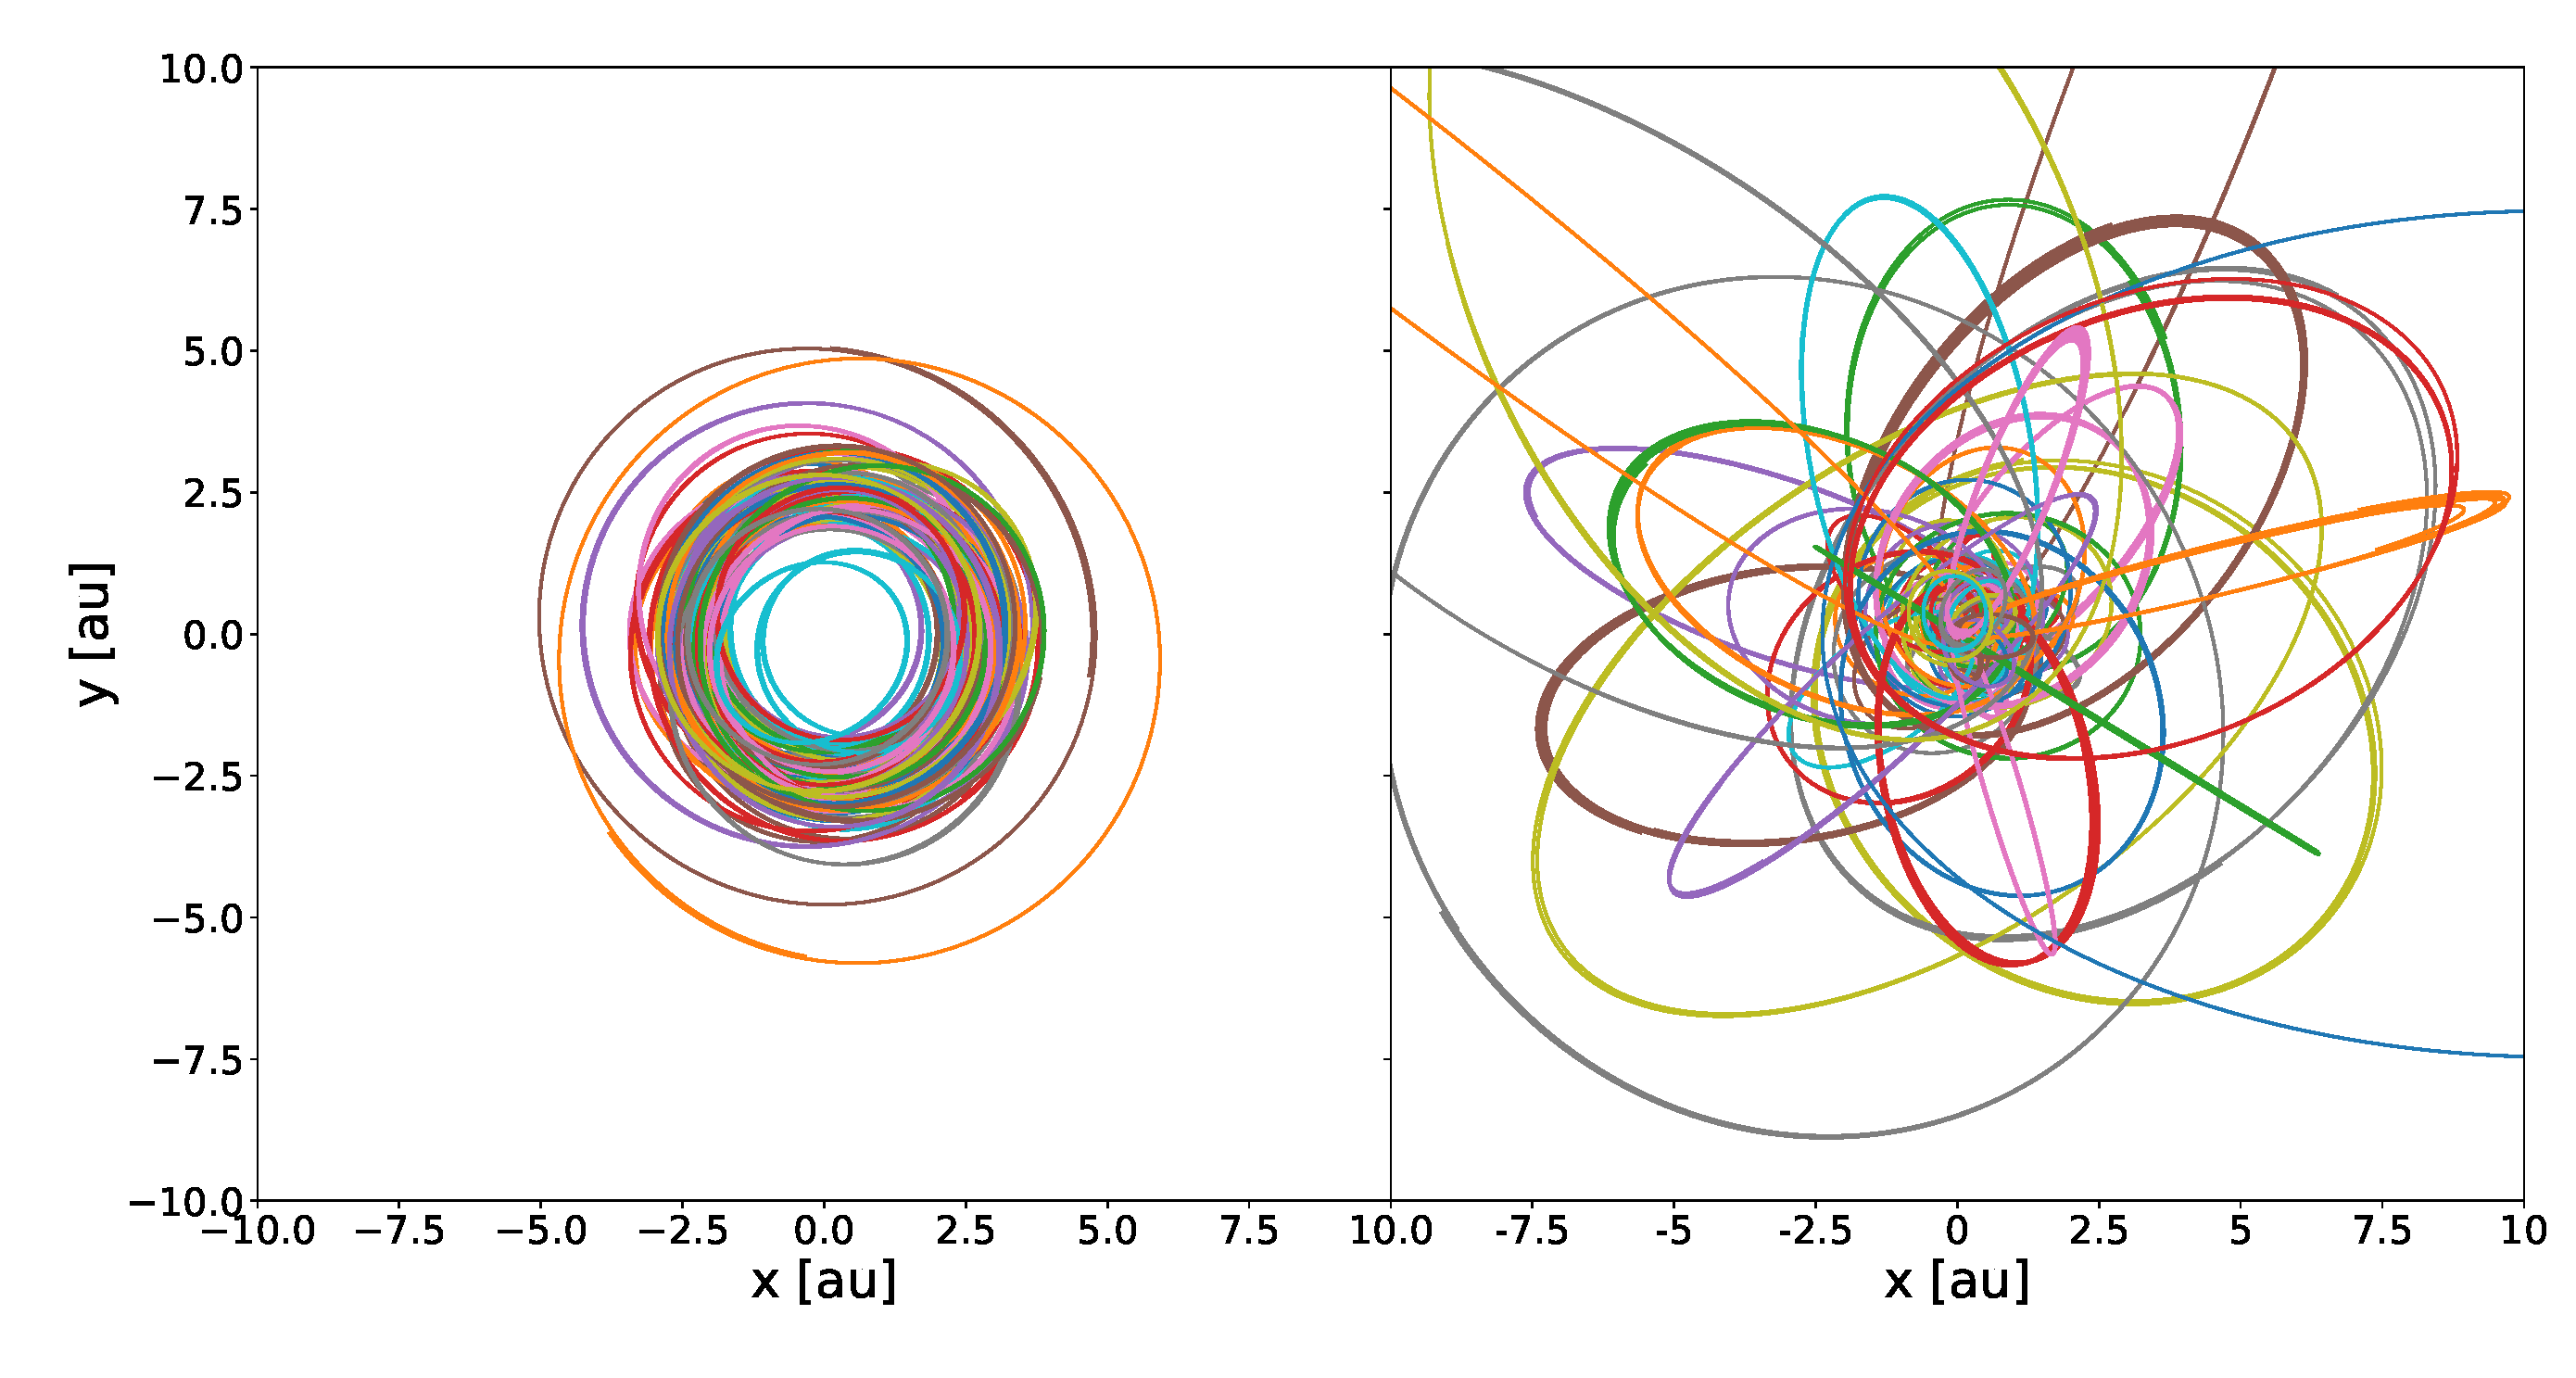
\includegraphics[width=170mm]{images/5_Trajectories.pdf}
	\centering
	\caption{\label{FIG:Object_Trajectories} Illustration of the difference between the trajectories of observed objects and known-impactors. Observed object are shown on the left while known-impactors are shown on the right. \textbf{Generally, the observed objects have circular orbits which lie flat in the orbital plane, while the known-impactors exhibit highly eccentric orbits at higher inclinations. These characterics, however, are not mutually exclusive and could be one the root causes of HOI's imperfect classification.}}
\end{figure*}

There are profound differences between the orbital elements of the two distinct populations of objects. Our artificial population of objects launched from Earth tend to have highly eccentric orbits distributed indiscriminately in space, whereas the observed objects tend to have circular orbits confined near the \textbf{ecliptic plane}. For the observed objects, the orbital plane is essentially empty within approximately 2\,au of the Sun, while for the KIs this is the most densely occupied space. This object distribution, however, should be expected considering that the all KIs were generated $1\pm0.017$\,au away from the Sun along the Earth's orbit.
                         
Plots of the semi-major axis versus the eccentricity are created for 2,000 KI, PI, and unidentified observed objects, which are shown below in figure \ref{FIG:AvsE}.
\begin{figure*}[h]
	\hspace*{-0.50cm}
	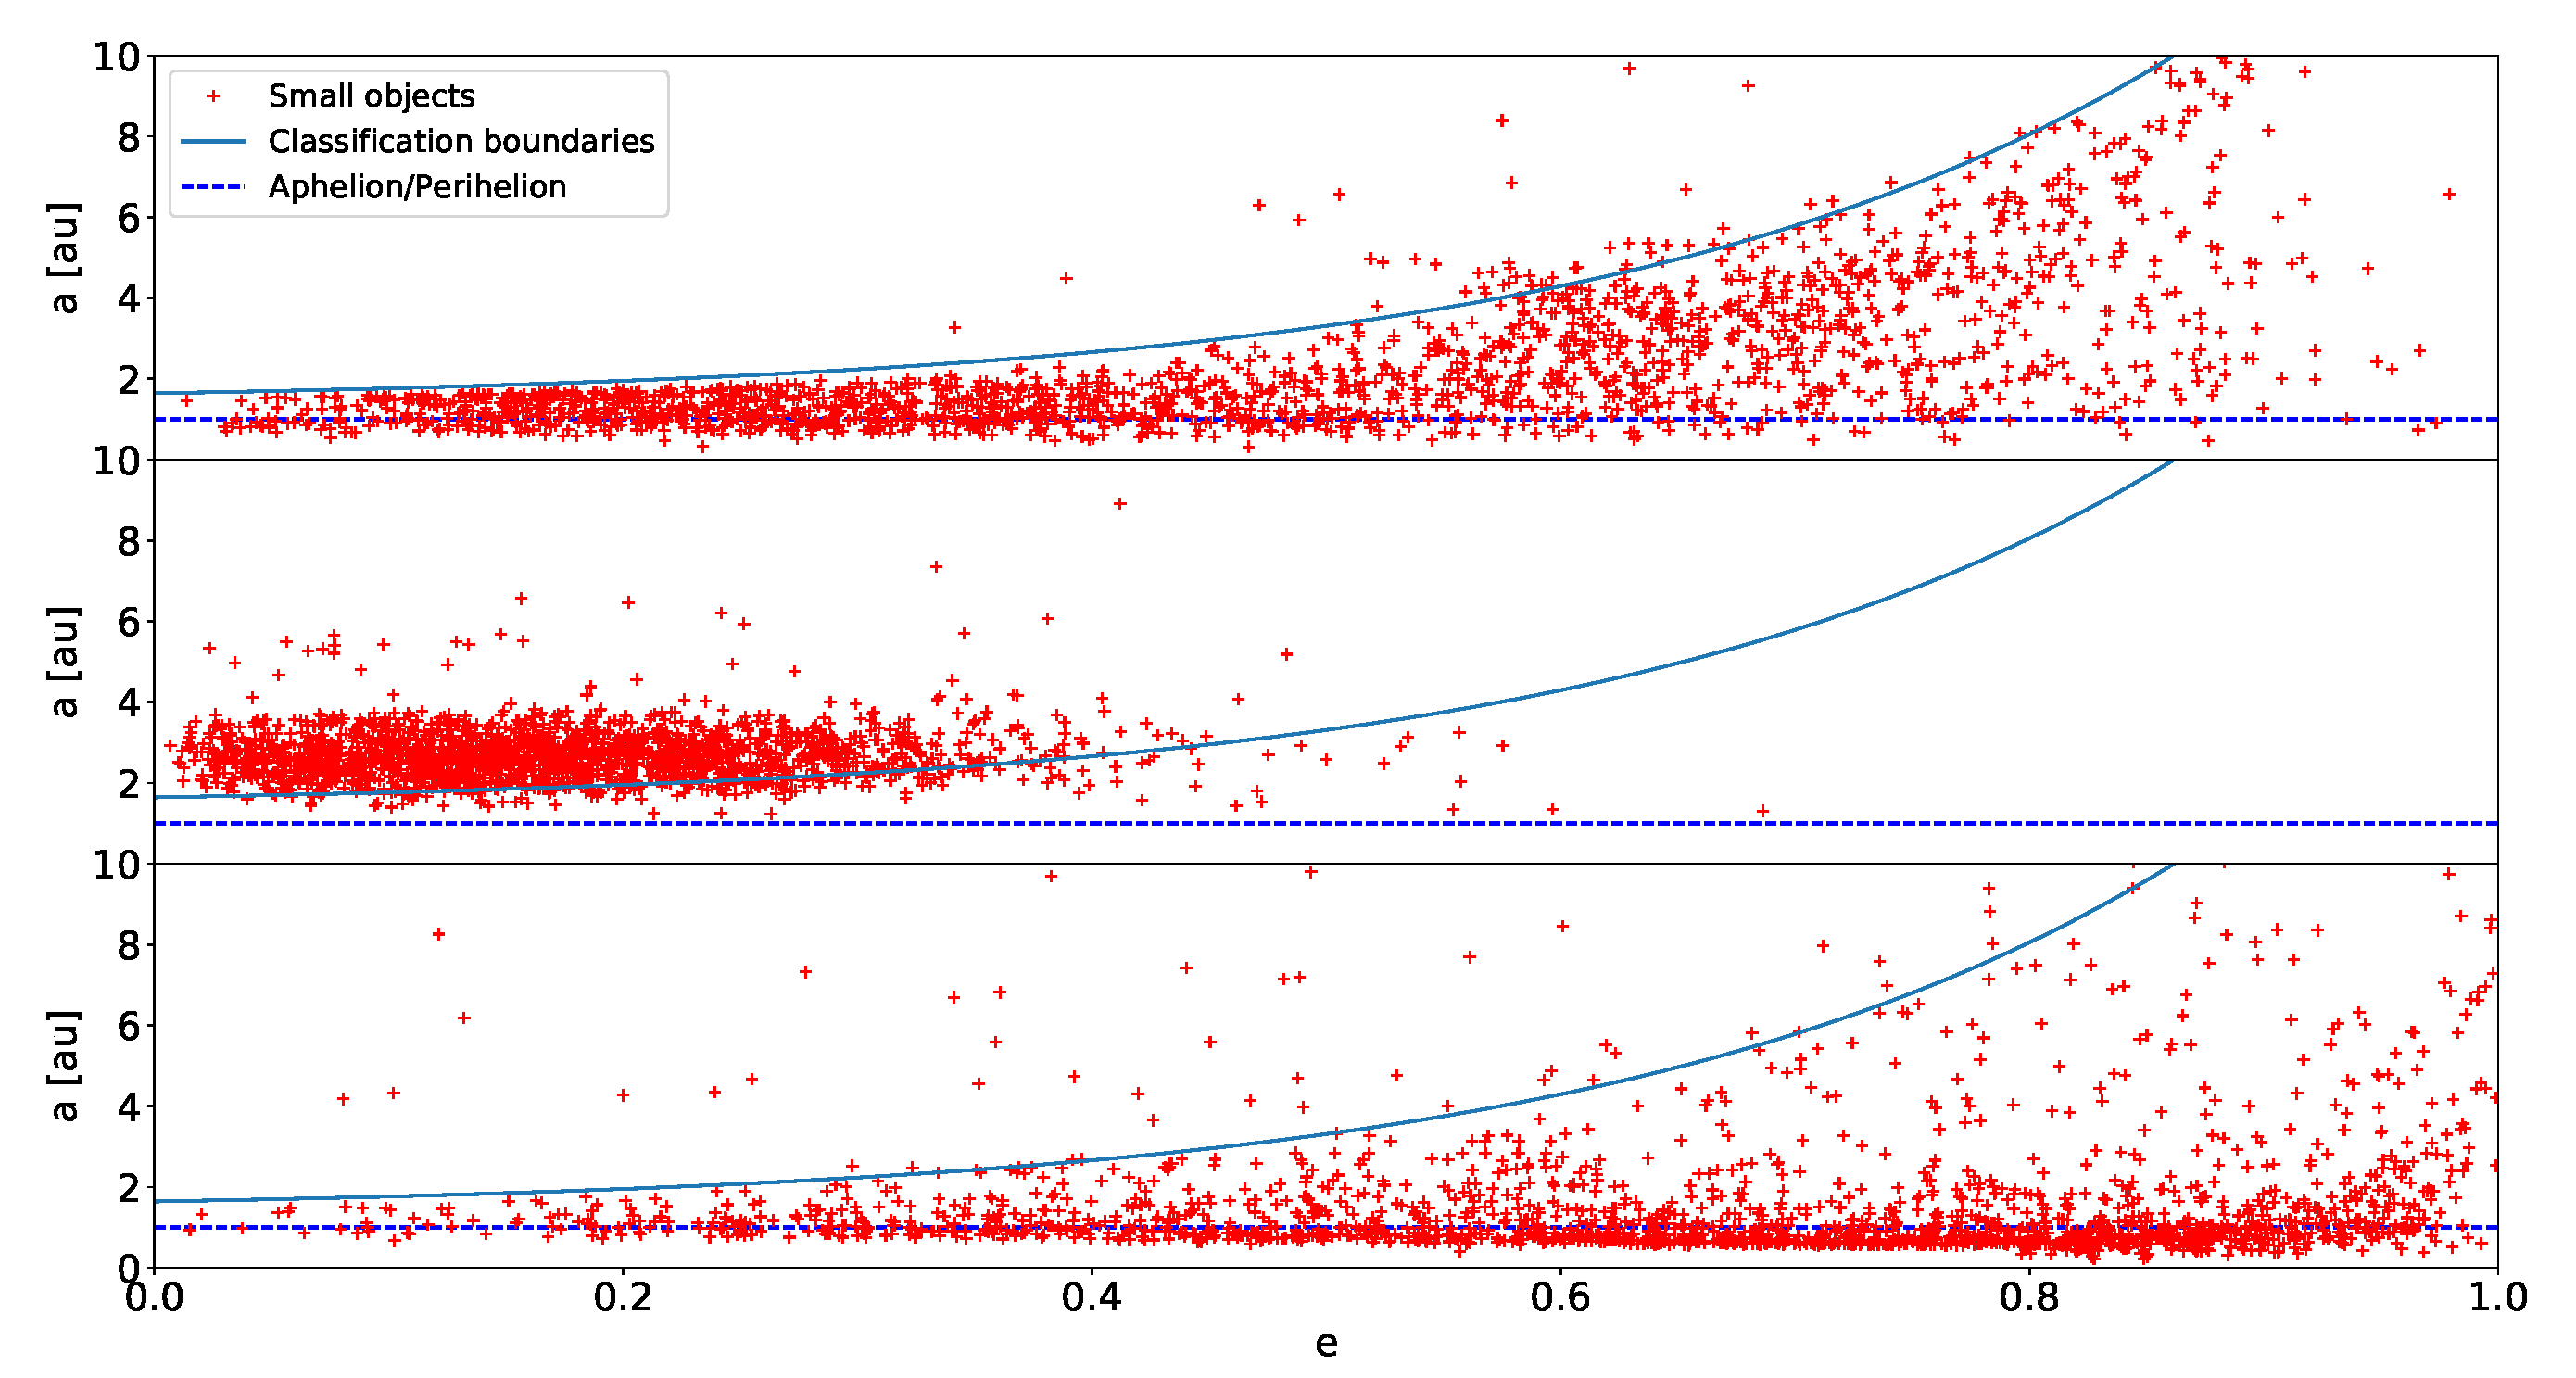
\includegraphics[width=170mm]{images/6_AvsE.pdf}
	\centering
	\caption{\label{FIG:AvsE} Display the semi-major axis versus the eccentricity for 2,000 PI, benign, and KI objects respectively top to bottom. The dotted blue lines represent the aphelion and perihelion distances of Earth's orbit and the teal curves represent the ``classification boundary'' \textbf{where} objects below are likely to be classified as PIs and those above are likely to be classified as benign.}
\end{figure*}
The \textit{a} versus \textit{e} ratio is an important factor in an object's identification. A curve is drawn to highlight an apparent ``classification boundary'', which is above 95.2\% of PI and below 90.3\% of unidentified observed objects. Although the boundary is an indicator of an object's potential classification, it is not definite, which is understandable considering that HOI takes 250 parameters as input for each object instead of just the \textit{a} and \textit{e} orbital elements at a single point in time. 

\section{Conclusions and Future Work}
\label{SEC:Conclusions}
Using HOI, we are able pick out 95.25\% of the known impactors (KIs) when mixed into the test set, and identify nearly nine-tenths of the PHOs and \textbf{virtually every asteroid that approached within 0.05\,au of Earth in our single-shot n-body simulations as PIs}. A short list is created of unacknowledged hazardous objects, which according to our simulations and filtering process, have a finite chance of striking Earth. Once trained, the network classifies an object as a PI or unidentified observed object in $2.3\times 10^{-4}$ seconds, which is a small fraction of time required for the Monte-Carlo method employed by NASA. 
 
 As mentioned in \S\,\ref{SEC:Results}, ideally, all PHOs should be identified, as they all come relatively close to Earth in the thousand-year simulations. Furthermore, 12.2\% of the PIs did not come within 0.5\,au of Earth within the time span of the simulations, which may imply that they pose no direct threat on the time scale considered. Both of these metrics indicate that the performance of HOI is still not optimal. To improve the network's classification accuracy, we suggest a few modifications. The labeling scheme could be improved, as not all observed objects are equally hazardous. A more intelligent labeling could be based on an object's closest approach to Earth. In addition, all of the object matrices represent a time span of 50 years, which may be an insufficient period to properly capture the secular changes in their orbital parameters. Increasing the time spans of the matrices could improve the predictability of HOI. 
\begin{acknowledgements}
We would like to thank the Microsoft Cooperation for the Azure research grant which made this work possible, and John thanks Sander van den Hoven for his mentoring during John's internship at Microsoft Amsterdam. This work was supported by the Netherlands Research School for Astronomy (NOVA), NWO (grant \# 621.016.701 [LGM-II]).

\end{acknowledgements}
\bibliographystyle{aa}
\bibliography{bibliography}

\end{document}


